\noindent The introduction section illustrated how the input is broken down to
yield a number of smaller and more manageable \emph{terms}, generally
corresponding to a single braket. Each of these \emph{terms} is fed into the algebraic
manipulator. This component of the program generates a set of instructions
for evaluating each of these \emph{terms}, which the task translator then converts into calls to the FCI
and linear algebra routines. Construction of this task list is split up into two major
parts; the tensor contraction task list generator, and the "gamma generator".
Before these individual components are discussed in detail it is
necessary to discuss the qualities the final task list should possess, and what
distinguishes and motivates the current approach. \\

\section{Core functionality}
\noindent At its core, the basic operation of the program is to evaluate terms such as 
\begin{equation}
\sum_{ijkl}\sum_{mnop} \sum_{IJ} \langle I | i^{\dagger}j^{\dagger}klm^{\dagger}n^{\dagger}op | J \rangle c^{M}_{I} c_{J}^{N} Y^{ML}_{ijkl}Z^{NP}_{mnop},
\label{eqn:generic_term}
\end{equation}
where $I$ and $J$ each denote a Slater determinant, and $L,M,N,P$ are state
indexes.  $\mathbf{Y}^{ML}$ and $\mathbf{Z}^{NP}$ are representations of
operators and $\hat{Y}$ and $\hat{Z}$ in the molecular orbital basis. For the time being
the state dependence of the operator representations will be ignored, but this has important consequences
for exploitation of symmetry, and will be discussed at length later. \\ 

\noindent The computational cost of directly evaluating terms such as (\ref{eqn:generic_term}) can be prove prohibitive,
particularly if the ranges of the indexes $i$, $j$, $k$, $l$, $m$, $n$, $o$, and $p$ are large (e.g., if they
range over virtual and core orbitals). The algebraic manipulator uses various commutation and symmetry relations
to rearrange expressions, such as (\ref{eqn:generic_term}), into a sum of terms in which
the orbital indexes only range over the active orbitals, e.g.,
\begin{equation*}
\sum_{stuvwxyz}\gamma_{stuvwxyz} A_{stuvwxyz}
+\sum_{stuvxy} \gamma_{stuvwx} A_{stuvwx}
\end{equation*}
\begin{equation}
+\sum_{stuv}\sum_{mnop} \gamma_{stuv} A_{stuv},
+\sum_{st} \gamma_{st}  A_{st}
+  A .
\label{eqn:A_list}
\end{equation}

\noindent Here the tensors $A_{ijkl...}$ are formed by performing 
contractions between and re-orderings of the indexes of tensors on $Y$ and $Z$ as 
determined from the commutation relations of the creation and annihilation operations, e.g.,
 
\begin{equation*}
A_{stwx} = \sum_{r}^{R}\hat{\wp}_{r}\sum^{c1}_{\{u,y\}}\delta_{uy}\sum^{c2}_{\{v,z\}} \delta_{vz}Y_{ijkl}Z_{mnop},
\end{equation*}

\noindent where the $c1$ and $c2$ are sets of pairs of indexes to be contracted, e.g.,
\begin{equation}
c2 = \{ \{i, k\} \} , \{j, k\} \} ,\{l, m\} \}.....\} 
\end{equation}
and $\hat{\wp}_{r}$ which transforms the ordered set of indexes
$\{u,v,s,t,w,x,y,z\}$ into some permutation, $r\in R$, of the ordered set of
indexes $\{i,j,k,l,m,n,o,p\}$, whilst also acting to multiply the result of the
summation by an appropriate factor.\\

\noindent The $\gamma$ and $\Gamma$ are defined by\footnote{It is worth noting that these are not normal ordered. The significance
of this will be explained in due course.}:
\begin{equation}
\gamma_{swtzuyvx} = \sum_{IJ} \langle I | s^{\dagger}wt^{\dagger}zu^{\dagger}yv^{\dagger}x | J \rangle c_{I} c^{*}_{J},
\end{equation}
\begin{equation}
\Gamma_{swtzuyvx}^{I} = 
\sum_{stuvwxyz} \sum_{J} \langle I | s^{\dagger}wt^{\dagger}zu^{\dagger}yv^{\dagger}x | J \rangle c^{*}_{J},
\end{equation}

\noindent A key feature of the program is that it is able to use decompose the $\mathbf{A}$ and $\mathbf{\gamma}$ objects
up into smaller sub-blocks, and use symmetries existing between these blocks, as well as number of other physical constraints
on the possibility of creation and annhilation operations, to inform the generation of the task list. Not only does this 
facilitate parallelization of the resulting task list, as operations concerning different blocks can be assigned to 
different nodes, but it may also substantially reduce the number of distinct operations which need to be performed. 
This kind of decomposition is particularly advantageous for relativistic systems, where the seperate treatment of
$\alpha$ and $\beta$ electrons can result in much larger tensors. For example, if the range of each index on
an eight index tensor is doubled, then the number of elements increases by a factor of 256.\\ 

\noindent The challenge faced by the algebraic manipulator is that whilst there
are several different series of form (\ref{eqn:A_list}) which are equal to
(\ref{eqn:generic_term}), these different series often differ wildly in the
amount of computational effort their evaluation requires. Hence the algebraic
manipulator must accomplish two things. First, it must decide on the series of
form (\ref{eqn:A_list}) that is least computationally expensive to evaluate.
Second, it must produce a sequence of instructions for evaluating the terms in
this series.  This second point may seem trivial, but is complicated
substantially by the decomposition of the tensors, and the need to take
advantage of symmetry in an effective manner\footnote{Whilst the algebraic
manipulator can also generate task lists for derivative expressions, the task
lists remain confined to evaluation of linear combinations of terms with one of
the following forms : 

\begin{equation}
\sum_{\substack{ijkl \\ mnop} }\gamma_{ijklmnop} A_{ijklmnop},
\text{ \ \ \ \ \ \ \ \ }
\sum_{ijkl}\gamma_{imjo} A_{imjoknlp},
\text{ \ \ \ \ or  \ \ \ \ }
\sum_{\substack{ijkl \\ mnop}}\Gamma^{I}_{ijklmnop} A_{ijklmnop}.
\label{eqn:kinds_of_terms}
\end{equation}
\noindent and the distinctions between these terms do not impact this preliminary discussion.}.\\

\noindent The algebraic manipulator accomplishes this by performing the operations as outlined in figure
\ref{fig:alg_manip_overview}. Both the $\mathbf{\gamma}$ tensors, as well as the
the tensors contracted to produce the $\mathbf{A}$ tensors, are split up into blocks. 
As calculation and storage of the $\mathbf{\gamma}$ and $\mathbf{\Gamma}^{I}$ is typically more
computationally demanding than obtaining the $\mathbf{A}$, minimization of the
number of distinct $\mathbf{\gamma}$ and $\mathbf{\Gamma}^{I}$ blocks
is prioritized, and each such block corresponds to a different task list, which
are typically evaluated seperately. \\

\begin{figure}[!ht]
\begin{center}
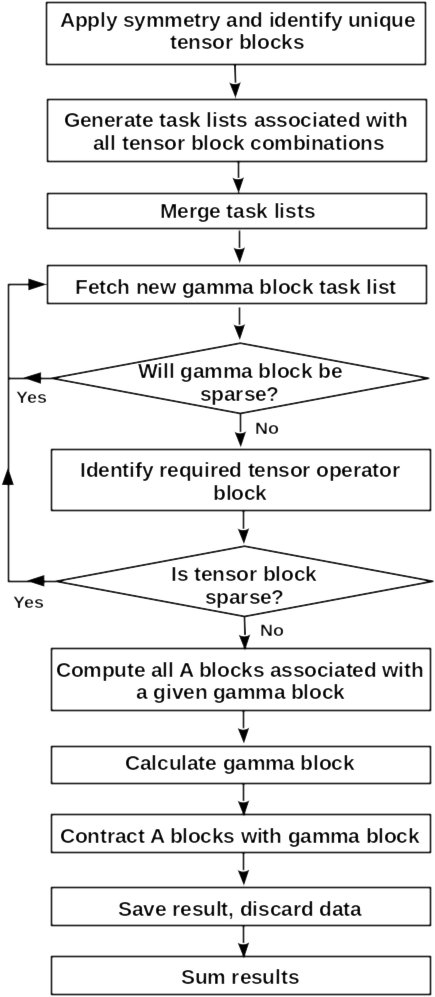
\includegraphics[width=0.6\textwidth]{alg_manip_over.png}
\caption{ Outline of the algebraic manipulator. }
\label{fig:alg_manip_overview}
\end{center}
\end{figure}

\noindent Chapter 5 focuses on the machinery (called the "gamma generator") for
chosing the the series of form (\ref{eqn:A_list}). Chapter 4 focuses on
evaluation of terms contained therein. The reason for this seemingly backwards
order is that the decisions made in the former and wholly dependent on the
factors governing the efficiency of the task lists generated in the latter.\\
